\chapter{Intel Architecture 32 bit, alcuni aspetti}
\label{cha:ia32}

\section{Bus e prime problematiche con la gerarchia delle memorie}
\label{sec:busMemorie}

Osserviamo la figura \ref{fig:strutturaInternaBus}; notiamo la presenza di due BUS principali, uno per la memoria (bus dati) e uno per le periferiche (IOB), separati da un \textit{bridge} fungente da ponte: si noti che essi hanno dimensione diversa (uno è a 64 bit, l'altro è a 8 bit). Ogni bus trasferisce una quantità di informazioni pari alla propria capacità ad ogni ciclo di clock, tuttavia non è detto che un singolo colpo di clock sia sufficiente per trasportare un intero dato. Prendiamo in considerazione le cosiddette "'linee di cache'"\footnote{Come nel caso delle memorie a livelli gerarchici superiori, anche la cache è suddivisa in blocchi di uguale dimensione. Nel caso delle cache questi blocchi sono detti \textit{linee di cache}. Nel Pentium e nel P6 (bus dati da 64 bit) la dimensione di ogni linea di cache è di 32 byte ed è identificabile dai 27 bit BA[31..5] (base) dell'indirizzo fisico costituito da 32 bit (27 bit base + 5 bit offset).}, unità grandi 32 byte in cui quest'ultima memoria è suddivisa: dovendo essere trasportate dal bus dati, si necessiterà di quattro cicli di bus per completare un singolo trasferimento. 

\begin{figure}[!h]
\centering
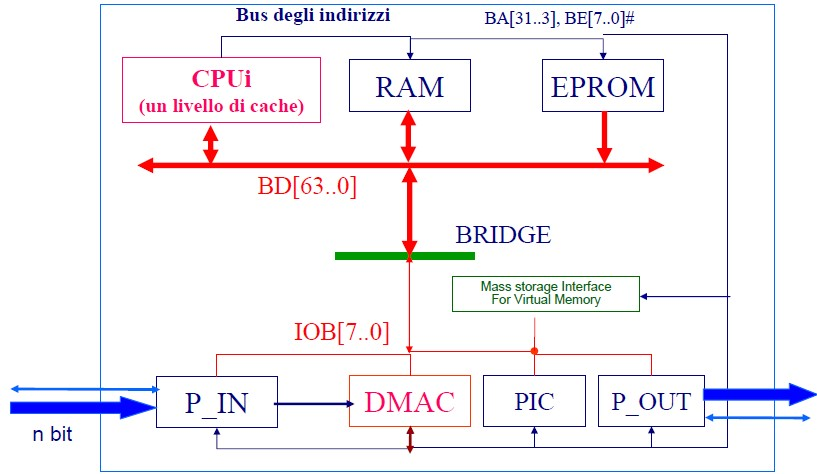
\includegraphics[width=0.85\columnwidth]{img/strutturaInternaBus}
\caption{Struttura interna della CPU}
\label{fig:strutturaInternaBus}
\end{figure}

Ogni ciclo di bus (dati), infatti, trasporta solo 8 dei 32 byte: da qui la necessità di effettuare cicli di bus multipli e di un segnale \textit{ready} (vedi fig. \ref{fig:segnaleReady}) in grado di indicare quando un dato è pronto e completamente trasferito. Inoltre, il meccanismo di generazione del segnale di \textit{ready} deve farci rispettare correttamente le tempistiche d'accesso alla memoria: se disponiamo, ad esempio, di una memoria con tempo d'accesso 100 ns e di un processore di 1 GHz dovremo aspettare 100 clock prima di poter effettuare le nostre operazioni.

\begin{figure}[!h]
\centering
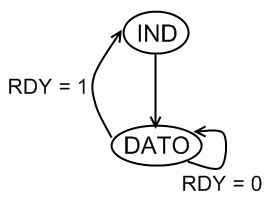
\includegraphics[width=0.35\columnwidth]{img/segnaleReady}
\caption{Funzionamento del segnale di \textit{ready}}
\label{fig:segnaleReady}
\end{figure}

Siamo quindi già arrivati a distinguere fra due diverse tipologie di cicli di bus:
\begin{itemize}
\item ciclo singolo: trasferiamo un unico dato;
\item ciclo \textit{burst}: trasferiamo quattro dati invece che uno solo (anche statisticamente si è visto che è la scelta migliore).
\end{itemize}
Purtroppo andare a leggere una periferica è un'operazione lentissima e abbiamo tempi d'accesso esorbitanti (confrontati con quelli d'accesso alla \textit{cache}); se il bus è bloccante ne segue che l'intera macchina lo è: volendo tuttavia poter usufruire dell'algoritmo di Tomasulo, il quale ci permette di eseguire fuori ordine, dobbiamo permettere che la memoria e l'I/O possano rispondere in ritardo (\textit{split transaction cycle}).

Inoltre, la CPU deve sapere a che ciclo di bus si riferisce un determinato dato: questo ci spinge ad inserire segnali di controllo e bit aggiuntivi. La cosa diventa ancora più complicata se abbiamo a che fare con sistemi \textit{multiprocessor}: dobbiamo infatti prevedere l'arbitraggio del bus, che è unico ed organizzato a mo' di \textit{pipeline} (cosicché serve dell'\textit{hardware} particolare per ogni stadio della pipeline e ulteriori segnali aggiuntivi... Non ne usciamo più!); infine possiamo avere in \textit{cache} delle copie di dati non consistenti (\textit{stail data}, dato presente in due memorie con valore diverso). Un analogo inconveniente può presentarsi per diversità dei dati fra la RAM e la \textit{cache} (problema di \textit{cache coherency}).
I componenti che si occupano di queste problematiche ed inoltre gestiscono le risorse, spegnendo la CPU in caso di emergenza o surriscaldamento, aumentando o riducendo la frequenza di \textit{clock}, etc\ldots sono i \textit{master} del bus (vedi fig. \ref{fig:busDintorni}.).

\begin{figure}[!h]
\centering
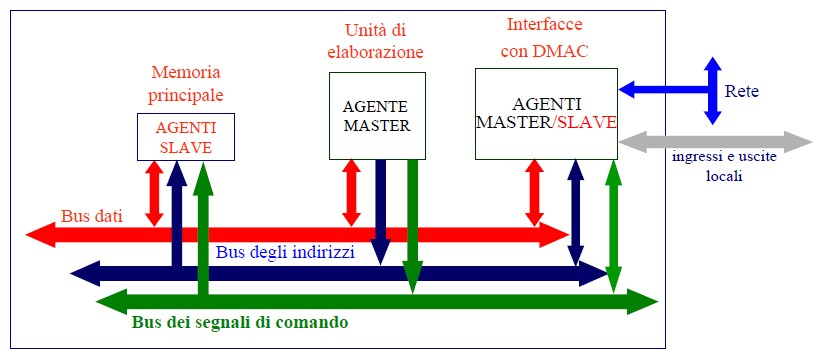
\includegraphics[width=0.75\columnwidth]{img/busDintorni}
\caption{Il bus e gli agenti interagenti con esso}
\label{fig:busDintorni}
\end{figure}

Morale della favola: un sistema complesso deve gestire moltissime cose e deve essere in grado di rilevare le occorrenze proibite, evitando che vengano eseguite e segnalando il \textit{software} con opportuni \textit{interrupt}\footnote{Prevenire è meglio che curare (cit.): serve obbligatoriamente un'opportuna \textit{routine} di gestione degli interrupt.}.

\section{IA32, protezione e gerarchia delle memorie}
\label{sec:gerarchia_memorie}

Osserviamo più da vicino al struttura del nostro processore Intel (vedi fig. \ref{fig:ia32}).

\begin{figure}[!h]
\centering
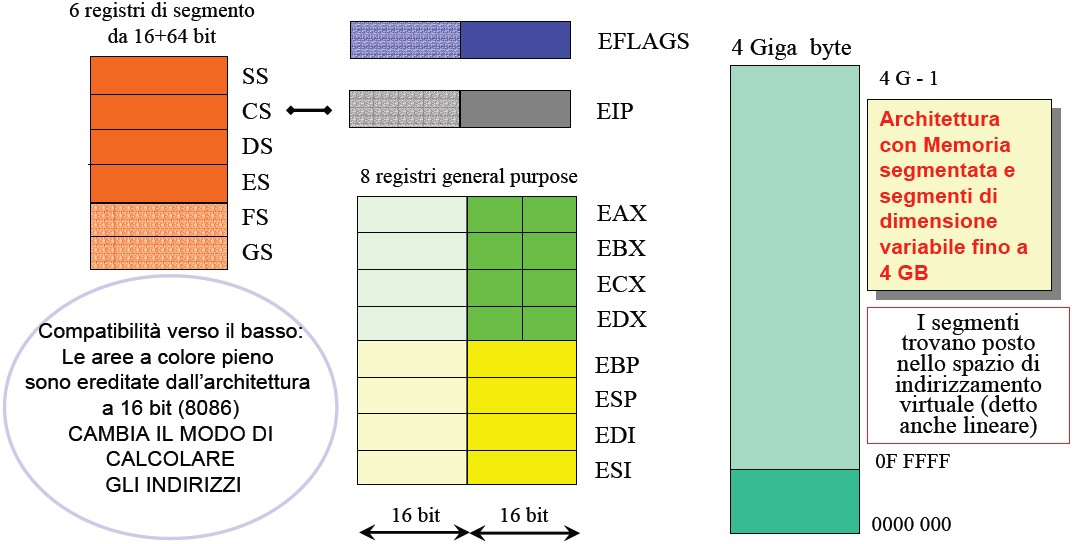
\includegraphics[width=\columnwidth]{img/IA32}
\caption{Ambiente di esecuzione di una applicazione
nell'architettura Intel a 32 bit.}
\label{fig:ia32}
\end{figure}

Qualche nota sui registri:
\begin{itemize}
\item ESP: \textit{Stack Pointer}. Si tratta dell'\textit{offset} nel registro di \textit{stack} dove siamo posizionati in un determinato momento;
\item EDI/ESI: registri indice per i vettori (max. 4 GB);
\item EIP: è l'\textit{Extended Instruction Pointer}, del quale presto scopriremo l'utilità;
\item sei registri di segmento entro i quali si manifesta la protezione\footnote{Una CPU protetta è una CPU in grado di separare i \textit{task} in base agli utenti che li hanno avviati.} della CPU (vedi capitolo \ref{cha:protezione}): essi indicano la tipologia, le proprietà, la dimensione e chi abbia il diritto d'accesso ad un certo segmento. Le CPU IA32 dispongono di sei registri di segmento: CS (\textit{code segment}: contiene il descrittore del blocco di codice in esecuzione), DS, ES, FS, GS ed SS (\textit{stack segment}: contiene il descrittore dello \textit{stack} in uso, v. paragrafo \ref{sec:controlliCPU}). La struttura di un registro di segmento è riportata in figura \ref{fig:regSegmento}.
\end{itemize}

Come nell'8086\footnote{Nell'8086 il \textit{Program Counter} era la coppia CS\#0000 + IP e puntava alla memoria di un 1 MB. Il PC era ottenuto da segmento + offset e si trovava in CS, con indirizzo iniziale FFFF0. In IA32, come si legge poco oltre, troviamo il descrittore di segmento, con indirizzo iniziale FFFFFFF0.}, per poter accedere a un segmento è necessario chi il relativo descrittore (per capire meglio cosa siano i descrittori si veda il paragrafo \ref{sec:descrittori}) sia stato preventivamente caricato in un registro di segmento. In particolare, CS contiene il segmento di codice del programma che in quel momento sta usando un'eventuale istruzione.

\begin{figure}[!h]
\centering
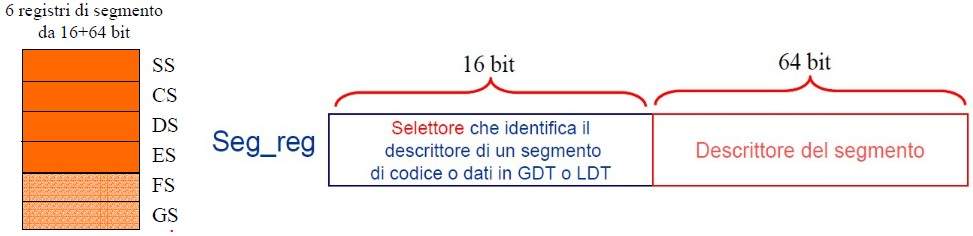
\includegraphics[width=0.84\columnwidth]{img/regSegmento}
\caption{Registro di segmento}
\label{fig:regSegmento}
\end{figure}

Nell'8086 ogni task ha 4 GB di memoria virtuale interamente dedicati a lui e sussistono sempre, anche se il quantitativo di RAM che ho nel sistema è molto inferiore: grazie a questo ingegnoso \textit{escamotage} siamo in grado di svincolare la dimensione del programma da quella della memoria fisica.

\begin{figure}[!h]
\centering
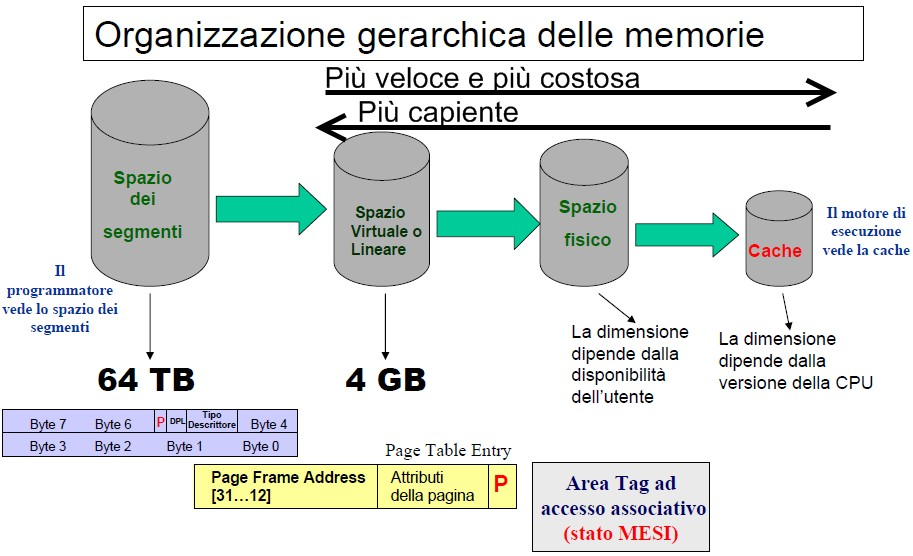
\includegraphics[width=\columnwidth]{img/slideSacra}
\caption{La gerarchia delle memorie}
\label{fig:slideSacra}
\end{figure}

A titolo informativo, mentre lo spazio dei segmenti e la \textit{cache} sono organizzati come matrici bidimensionali (a 2 coordinate), la memoria virtuale è lineare (1 coordinata).

Vediamo ora qualche esempio di codice in linguaggio macchina (NOTA: nei compiti segmento di codice, di dati e di \textit{stack} costituiscono un trinomio obbligatorio da definire!). \\
Segmento di \textbf{codice}:
\begin{verbatim}
             ER@10000H
Entry point: MOV DS, SEG_DATI
             ADD AL, DS:5 (aggiunge 5 ad AL)
             MOV DS: ALFA, AL 
             MOV EDI, 0 (mette a 0 EDI)
             MOV DS: BETA(EDI), EBX
             PUSH ...
             CALL ... (servirà supporto per il nesting!)
\end{verbatim}
Segmento \textbf{dati}:
\begin{verbatim}
         SEG_DATI SEGMENT RW@8000H (RW => leggere/scrivere)
8000H |  ALFA DB (DB => define byte)
8001H |  BETA DD 4DUP    (DD => double word = 4 byte)
...   |                  (4DUP => serve a duplicare 4 volte qualcosa)
      |                  (4 byte x 4 = 16 = 10H in esadecimale!)
8011H |  GAMMA DB
...
         ENDS
\end{verbatim}
Segmento di \textit{\textbf{stack}}:
\begin{verbatim}
STK_SEGMENT <..., ...>
\end{verbatim}

Notiamo che:
\begin{itemize}
\item la variabile ALFA è individuata dall'indirizzo logico <SEG\_DATI, 0>;
\item la variabile BETA(0) è individuata all'indirizzo logico <SEG\_DATI, 1>;
\item la variabile BETA(1) è individuata all'indirizzo logico <SEG\_DATI, 5>. Il 5 è stato calcolato ricordando che ogni elemento della struttura dati BETA è una \textit{double word} (4 byte);
\item gli indirizzi 8000H, 8001H, etc\ldots non sono indirizzi logici ma indirizzi nello spazio virtuale.
\end{itemize}

\begin{figure}[!h]
\centering
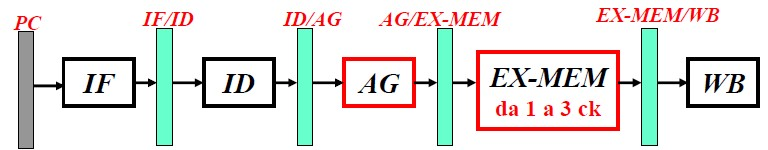
\includegraphics[width=0.8\columnwidth]{img/pipelineIndirizzi}
\caption{Pipeline e generazione degli indirizzi.}
\label{fig:pipelineIndirizzi}
\end{figure}

La pipeline come pensata in figura è in grado di funzionare su macchine M-R (come quelle Intel) e di effettuare la traduzione fra indirizzo logico e indirizzo virtuale. Ad esempio, ALFA ha indirizzo logico\footnote{Il programmatore (e i compilatori) vedono uno spazio di indirizzamento segmentato, il che significa che ogni istruzione e ogni dato vengono localizzati attraverso una coppia di coordinate: il segmento di appartenenza e la posizione (offset) all'interno del segmento (come in IA16); l'offset nel segmento può essere determinato dal compilatore (es. etichetta o variabile) oppure calcolato a \textit{runtime} (es. indirizzamento tramite registro base e registro indice).
} <SEG\_DATI, 0> ma indirizzo virtuale 8000H (+ offset pari a 0) calcolato facendo l'usuale operazione di somma base\footnote{DS concatenato con 4 zeri nell'8086; nell'IA32 è l'indirizzo virtuale calcolato nello stadio di AG, all'interno del quale è necessariamente utile avere i registri di segmento.} + offset.

\subsection{I \textit{Page Fault} e il reperimento dei blocchi}
\label{sec:pageFault}

Ogni volta che si esegue un \textit{task} è come se esistesse un file, all'interno dell'hard disk e grande 4 GB (ma magari "'scritto'" anche solo in pochi KB), che viene portato in memoria fisica (RAM): siccome la dimensione della RAM può essere anche molto inferiore a 4 GB, tale file viene smembrato in blocchi tutti uguali (pagine) di dimensione 4 KB. Se in memoria fisica viene ricercata una pagina che non c'è, allora si genera un \textit{page fault}, al quale si risponde caricando i dati cercati da memoria virtuale a memoria fisica.
La CPU, quando deve cercare qualcosa nella \textit{cache}, controlla i primi 27 bit dell'indirizzo fisico\footnote{Si ricorda che 27 dei 32 bit rappresentano la base e i 5 rimanenti l'offset.}.

\begin{figure}[!h]
\centering
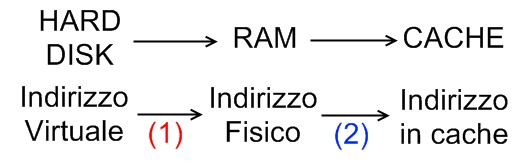
\includegraphics[width=0.6\columnwidth]{img/hdrc}
\caption{Indirizzi e rispettive locazioni}
\label{fig:hdrc}
\end{figure}

La traduzione degli indirizzi (vedi fig. \ref{fig:hdrc}) avviene attraverso tabella associativa (passaggio indicato col numero 1, IF-IC) oppure attraverso un \textit{Translation Look-Aside Buffer} (passaggio 2, IV-IF).
L'assenza di una pagina in memoria può avvenire ad ogni livello:
\begin{itemize}
\item \textit{page fault} (tra IV e IF);
\item \textit{miss} (tra IF e IC);
\item \textit{segment non present fault} (tra IL e IV).
\end{itemize}
Ovviamente l'architettura che gestisce tutte queste tipologie di \textit{miss} dev'essere adeguatamente veloce e deve sussistere una collaborazione HW-SW per gestire:
\begin{enumerate}
\item i \textit{cicli burst} per portare i dati in \textit{cache};
\item l'allocazione delle pagine in memoria centrale, attività della quale si occupa in genere il sistema operativo;
\item il reperimento delle informazioni non ancora presenti in memoria virtuale (\textit{segment non present fault});
\item il controllo sugli accessi in memoria (protezione);
\item la definizione di processi e delle risorse di memoria ad essi associati;
\item la separazione tra processi (protezione);
\item la commutazione tra un processo e l'altro (\textit{task switching});
\item le tecniche d'accesso all'hard disk, che è risaputamente un collo di bottiglia per le prestazioni.
\end{enumerate}
Tutto ciò (soprattutto i punti 1, 2, 3 e 8) è causa una gran mole di \textit{overhead}, ma fortunatamente il numero di \textit{miss} non è così grande grazie al principio di località.

\section{Descrittori di segmento}
\label{sec:descrittori}

Tutto quello che abbiamo detto sta in piedi se disponiamo di alcune informazioni importanti:
\begin{itemize}
\item a che livello è mappato il blocco di dati?
\item a che indirizzo?
\item quanto è grande?
\item è presente o devo trasferirlo?
\end{itemize}
Tutti questi particolari sono ben annotati nei cosiddetti \textit{descrittori}. Nell'architettura IA32 i descrittori hanno una struttura come indicato in figura \ref{fig:descrittoreGenerico}.

\begin{figure}[!h]
\centering
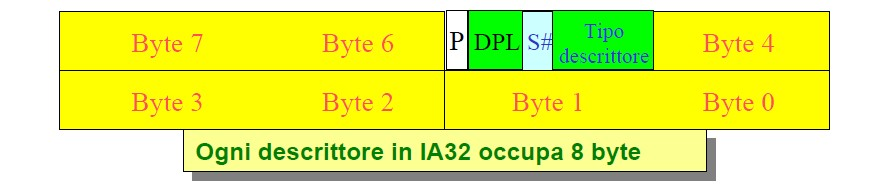
\includegraphics[width=0.75\columnwidth]{img/descrittoreGenerico}
\caption{Struttura generica di un descrittore}
\label{fig:descrittoreGenerico}
\end{figure}

Ad ogni segmento è associato un descrittore di 8 byte contenente tutti gli attributi del segmento (indirizzo di origine, lunghezza del segmento, diritti di accesso, tipo, etc\ldots). Per accedere a un oggetto in memoria è necessario conoscere il segmento di appartenenza; il relativo selettore deve essere caricato in un registro di segmento i quali sono sei\footnote{Quindi in ogni istante il programma ha la visibilità di non più di sei segmenti.}.

In IA32 la dimensione massima di un segmento è 4 GB; all'interno del descrittore sono contenute le informazioni necessarie per verificare se un accesso al segmento è lecito e in tal caso indica dove il segmento si trova.
Il linguaggio macchina delle CPU da 32 bit è un'estensione di quello dei processori 8086/88: così come questi due ultimi processori avevano una memoria segmentata, così anche per l'architettura a 32 bit ad ogni segmento è associato un \textit{descrittore di segmento} (vedi fig. \ref{fig:descrittoreSegDati}). Il descrittore va caricato in un registro di segmento, così come andava caricato in DS l'indirizzo iniziale del segmento in IA16\footnote{Data l'istruzione \textit{assembler} (ALFA è l'offset):\\
\texttt{MOV AL, ES:[ebx + edi].ALFA }\\
L'indirizzo virtuale è calcolato così:\\
\texttt{IV = ES.base\_seg + EBX + EDI + ALFA}\\
In generale, l'indirizzo virtuale (o lineare) di un operando in memoria in IA32 è infatti:\\
\texttt{IV = seg\_reg.base\_seg + EA}}.

\begin{figure}[!h]
\centering
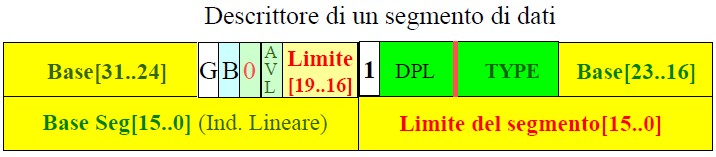
\includegraphics[width=0.75\columnwidth]{img/descrittoreSegDati}
\caption{Descrittore di un segmento dati}
\label{fig:descrittoreSegDati}
\end{figure}

In generale nell'architettura IA32 i descrittori vengono utilizzati non solo per descrivere e gestire i segmenti di codice e dati, ma anche per descrivere e gestire altri tipi di oggetti detti \textit{oggetti di sistema}\footnote{Il bit S\# definito nel byte 5 del descrittore consente di specificare se tale descrittore descrive un oggetto di sistema (S\# = 0) o un oggetto dell'applicazione (S\# = 1).
Gli oggetti dell'applicazione sono suddivisi in:
\begin{itemize}
\item segmenti di codice;
\item segmenti di dati e/o \textit{stack}.
\end{itemize}
Gli oggetti di sistema suddivisi in:
\begin{itemize}
\item segmenti contenenti i descrittori di task detti TSS o \textit{Task
State Segment};
\item porte di accesso a task e procedure di servizio dette \textit{Gates}
(i \textit{Gates} controllano sia l'accesso eseguito a controllo di
programma, sia l'accesso eseguito in risposta a eventi
interni o esterni);
\item tabelle con l'elenco degli oggetti accessibili a un task (\textit{Local
Descriptor Table} o LDT).
\end{itemize}
}

I descrittori sono radunati in apposite tabelle dette \textit{tabelle dei descrittori} (\textit{Global Descriptor Table}, GDT, \textit{Local Descriptor Table}, LDT), come illustrato in figura \ref{fig:sedeDescrittori}. È possibile accedere a un descrittore attraverso una chiave di accesso di 16 bit (detta selettore, la cui struttura è riportata in figura \ref{fig:strutturaSelettori}) contenente sia l'identificatore della tabella (GDT o LDT) sia l'indice del descrittore nella tabella (13 bit). Entrambe le tabelle contengono al massimo 8192 elementi di 8 byte.

\begin{figure}[!h]
\centering
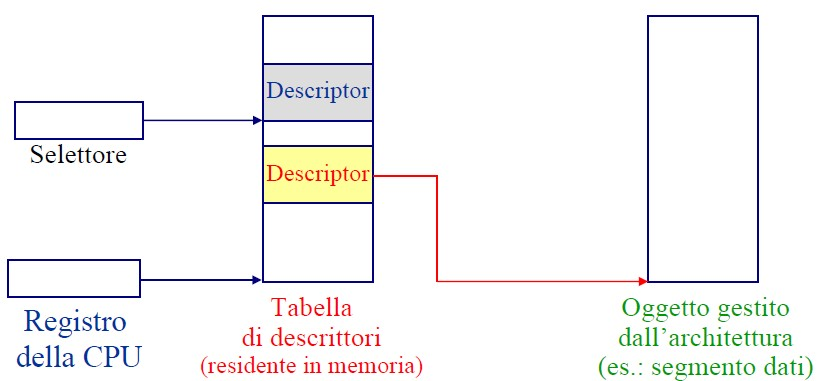
\includegraphics[width=0.75\columnwidth]{img/sedeDescrittori}
\caption{Locazione dei descrittori}
\label{fig:sedeDescrittori}
\end{figure}

\begin{figure}[!h]
\centering
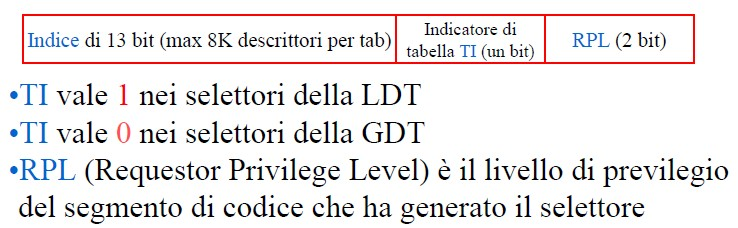
\includegraphics[width=0.75\columnwidth]{img/strutturaSelettori}
\caption{Struttura dei selettori}
\label{fig:strutturaSelettori}
\end{figure}

I descrittori sono parecchi: ve n'è un tipo per i segmenti di dati, uno per i segmenti di codice, uno per i \textit{task}, etc\ldots Per questo esiste anche un identificatore del tipo di descrittore: esso consta di 5 bit, dei quali solo 4 vengono in realtà usati (il primo è fisso ad 1), per un totale di 16 possibili oggetti all'interno della CPU.

\subsection{Descrittore di dato}
\label{sec:descrittoreDato}

\begin{figure}[!h]
\centering
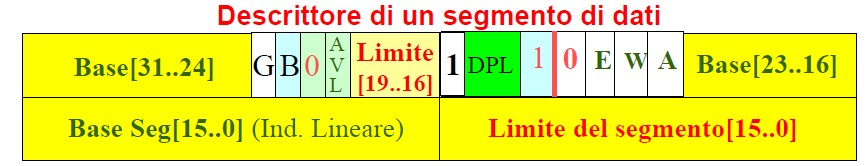
\includegraphics[width=0.75\columnwidth]{img/segDati}
\caption{Descrittore di dato}
\label{fig:segDati}
\end{figure}

In questo descrittore (vedi fig. \ref{fig:segDati}):
\begin{itemize}
\item DPL è il livello di privilegio del segmento associato al descrittore (\textit{Descriptor privilege level});
\item il bit più significativo del campo "'tipo descrittore'" discrimina tra segmenti di dato e segmenti di codice;
\item il bit A (\textit{Accessed}) è resettabile dal software e viene settato automaticamente ogni volta che viene fatto un accesso al segmento (cioè ogni volta che il descrittore viene caricato su un registro di segmento);
\item il bit E (\textit{ExpandDown}) definisce un segmento dati per il quale il limite è l'indirizzo più basso del segmento (segmento di \textit{stack} che cresce verso indirizzi decrescenti);
\item la base del segmento (per esempio l'indirizzo iniziale del segmento in uno spazio di indirizzamento lineare di 4GB) è memorizzato nei byte 2, 3, 4, 7 (vedi fig. \ref{fig:descrittoreGenerico}). Lo spazio di indirizzamento lineare può essere la memoria fisica o la memoria virtuale;
\item il limite del segmento è un campo di 20 bit memorizzato nei byte 0 e 1 e nei bit [0..3] del byte 6 (vedi fig. \ref{fig:descrittoreGenerico}); nei segmenti di codice e nei segmenti dati con E = 0 l'indirizzo base + limite è l'indirizzo lineare più alto del segmento associato al descrittore. Nei segmenti dati con E = 1, invece, sono vietati tutti gli accessi a indirizzi compresi tra base e base + limite;
\item anche se il campo limite è di 20 bit, la dimensione massima di un segmento non è limitata a un MB, ma può essere anche di 4 GB, infatti l'unità di misura di questo campo può essere il byte o la pagina di 4 KB; chi definisce l'unità di misura è il bit G (\textit{granularity});
\item bit G (\textit{Granularity}): se G = 0, il limite è espresso in byte; se G = 1 il limite è espresso in pagine di 4KB;
\item il bit B riguarda la gestione dei segmenti di \textit{stack}: se B = 1 lo \textit{stackpointer} è di 32 bit (ESP) e l'offset massimo è 0F FFFF FFFH, altrimenti lo \textit{stackpointer} è di 16 bit (SP) e l'offset massimo è 0F FFFH;
\item il bit AVL è un bit disponibile (\textit{available}) a chi scrive il sistema operativo;
\item il bit P (\textit{Present}, vedi fig. \ref{fig:regSegmento}, nella \ref{fig:segDati} è ad 1) indica se il segmento è mappato nel livello adiacente della gerarchia delle memorie (cioè se è mappato in memoria virtuale).
\end{itemize}


\subsection{Descrittore di codice}
\label{sec:descrittoreCodice}

\begin{figure}[!h]
\centering
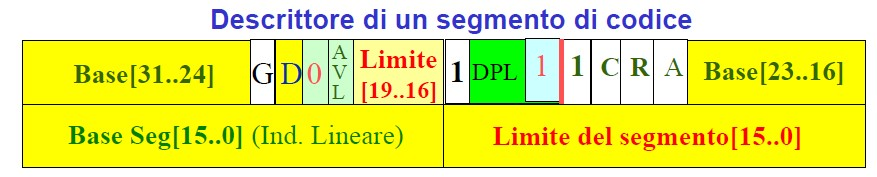
\includegraphics[width=0.75\columnwidth]{img/segCodice}
\caption{Descrittore di codice}
\label{fig:segCodice}
\end{figure}
Oltre ad alcuni attributi illustrati nel paragrafo \ref{sec:descrittoreDato}, abbiamo (vedi fig. \ref{fig:segCodice}).
\begin{itemize}
\item il bit W (\textit{Writable}) stabilisce se un segmento dati è di tipo \textit{Read/Write} o \textit{Read Only};
\item bit D nei segmenti di codice vale 1 se il codice è scritto nel linguaggio macchina della IA-32, mentre vale 0 se si tratta di codice macchina del processore 8086 (in particolare operandi e offset di 16 bit);
\item il bit R (\textit{Readable}) stabilisce se un segmento di codice è di tipo \textit{Execute/Read} o \textit{Execute Only}, cioè se contiene anche dati o è solo eseguibile;
\item il bit C (\textit{Conforming}) di un segmento di codice indica che il livello di privilegio a cui il segmento viene fatto eseguire è quello del codice che ha messo in esecuzione il segmento stesso (il segmento cioè eredita il livello di privilegio del codice chiamante).
\end{itemize}

Si ricorda che il descrittore di codice corrente è contenuto nel registro CS del nostro microprocessore.

\section{Politiche d'avvio e descrittori}
\label{sec:avvioDescrittori}

\begin{figure}[!h]
\centering
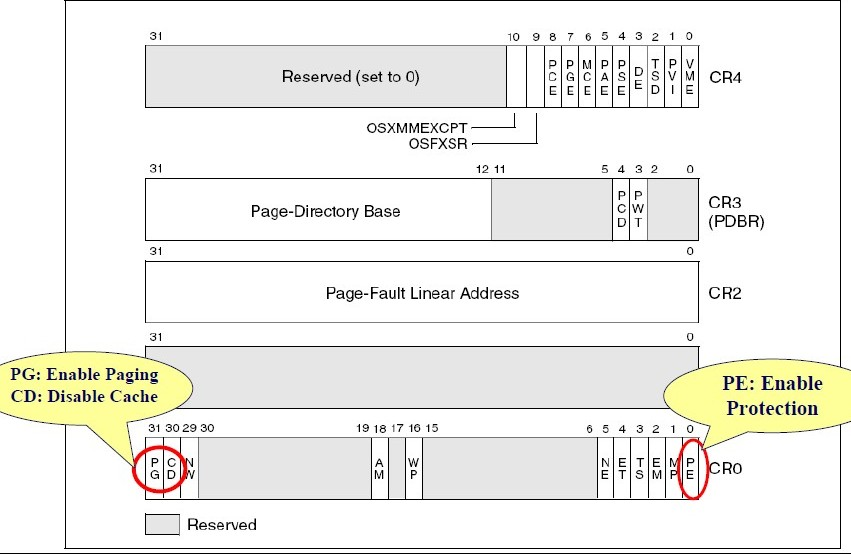
\includegraphics[width=0.9\columnwidth]{img/PGeRegistri}
\caption{I registri di controllo della CPU e l'abilitazione dei diversi livelli della gerarchia delle memorie}
\label{fig:PGeRegistri}
\end{figure}

La memoria, all'accensione della macchina, deve partire con i descrittori (e relative tabelle) già pronti: a tal proposito, le tabelle vanno portate nella memoria (vergine) non appena viene fatto partire il nostro dispositivo. Mentre però viene effettuato lo \textit{start-up}, la CPU si comporta come un 8088 (che non aveva i descrittori e quindi può benissimo funzionare senza!) e fa uso di un registro (CR0, vedi figura \ref{fig:PGeRegistri}) che si occupa di gestire il transitorio in cui non si ha alcuna tabella. Il bit PE (\textit{Protection Enable}) è pari a 0 durante tutta la transizione e va ad 1 quando finalmente tutto è pronto per funzionare a regime\footnote{Se PG=0 la memoria virtuale è disabilitata quindi l'indirizzo si riferisce alla memoria fisica. Se PG=1 la memoria virtuale è abilitata e gli indirizzi fanno riferimento alla memoria virtuale (in particolare il registro BASE SEG).}.

Mentre la CPU si accende, la \textit{cache} è disabilitata (CB=1) e anche l'impaginazione (PG=0) lo è: ufficialmente, sotto quest'ultimo punto di vista, tutto funziona come nell'IA16.
Abilitata \textit{cache} e impaginazione, dispongo della gerarchia completa delle memorie.

\section{Ciclo IDLE e considerazioni sui consumi}
\label{sec:idleConsumi}

Il ciclo \textit{idle} (vedi fig. \ref{fig:halt}) è attivo quando la CPU ha ben poco da fare: durante il suo svolgimento, la CPU va in HALT per cercare di spegnere quasi tutto e - di conseguenza - di consumare il meno possibile. I consumi di un moderno elaboratore possono infatti essere suddivisi in tre parti, più o meno equivalenti come dispendio:
\begin{itemize}
\item la CPU;
\item le periferiche (HD, monitor, etc\ldots);
\item tutto il resto (memorie, bridge, etc\ldots).
\end{itemize}

\begin{figure}[!h]
\centering
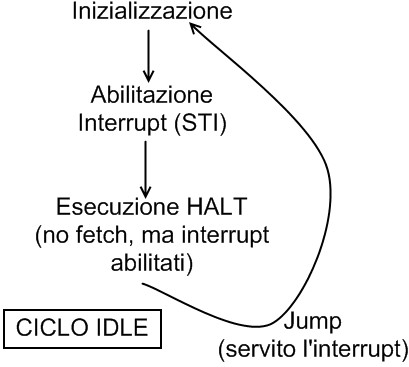
\includegraphics[width=0.55\columnwidth]{img/halt}
\caption{Struttura del ciclo \textit{idle}}
\label{fig:halt}
\end{figure}

Spegnendo la CPU abbatto i consumi di 1/3; altri accorgimenti per il risparmio dell'energia possono essere l'utilizzo della modalità \textit{standby}, lo spegnimento dell'\textit{hard-disk}, l'inibizione \textit{totale} del clock alla CPU o, infine, la riduzione della frequenza di funzionamento o della tensione\footnote{Servirà ovviamente un sistema di monitoraggio per decidere come modulare questi due parametri in base alla situazione.} in virtù della relazione
\[
P=KV^2f
\]
(con $K$ costante di proporzionalità, $V$ tensione e $f$ frequenza).

Ebbene, quando la CPU è in HALT viene generato un apposito ciclo di bus (che viene visto anche dal bridge) e che fa partire un \textit{timer} il quale, allo scadere, priva la CPU del clock.
Se togliamo anche l'alimentazione, la CPU passa in modalità \textit{deep sleep} (sonno profondo), in cui è il bridge a gestire gli \textit{interrupt}: il risveglio sarà lentissimo, ma almeno avremo risparmiato moltissima energia.

